\documentclass[b5paper]{scrbook}

\usepackage{lipsum}
\usepackage{afterpage}
\usepackage{rotating}
\usepackage[x11names]{xcolor}

\begin{document}
	
	\tableofcontents
	\pagestyle{plain}
	
	% \afterpage{\clearpage}
	\begin{sidewaysfigure}[ht]
		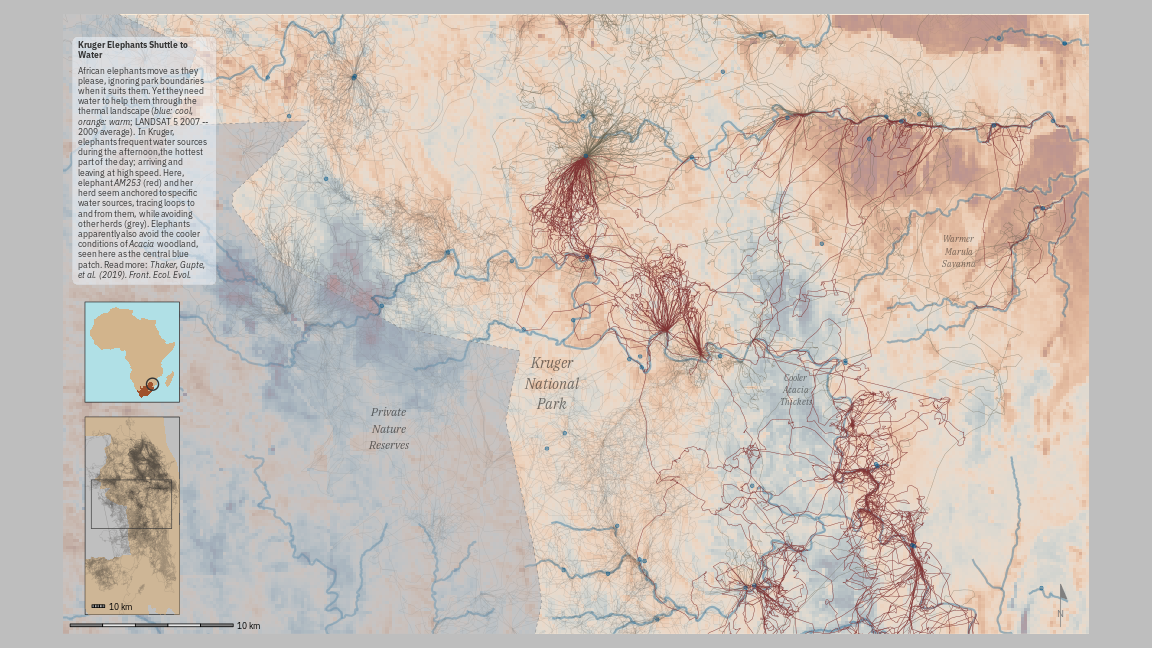
\includegraphics[width=1.2\textwidth,align=cb]{../figures/boxes/elemove.png}
		\label{fig:LandscapeFigure}
	\end{sidewaysfigure}
	
	\begin{addmargin}[-1cm]{-2cm}
		\colorbox{Snow2}{
			\begin{minipage}[t]{\linewidth}%{\dimexpr\linewidth-2\fboxsep}
				%\phantomsection
				% \addtocontents{toc}{\protect\vspace{\beforebibskip}}%
				\addcontentsline{toc}{chapter}{\tocEntry{\color{gray}\bfseries{Mapping Animal Movement in \textit{R}}}}%
				%\chapter*{Mapping Animal Movement in \textit{R}}
				\chaptermark{Mapping Animal Movement in \textit{R}}
				
				\paragraph{Something}
				\lipsum[1]
			\end{minipage}
		}	
	\end{addmargin}

\end{document}
